\scanpage{30}
\margin{29}
\figure{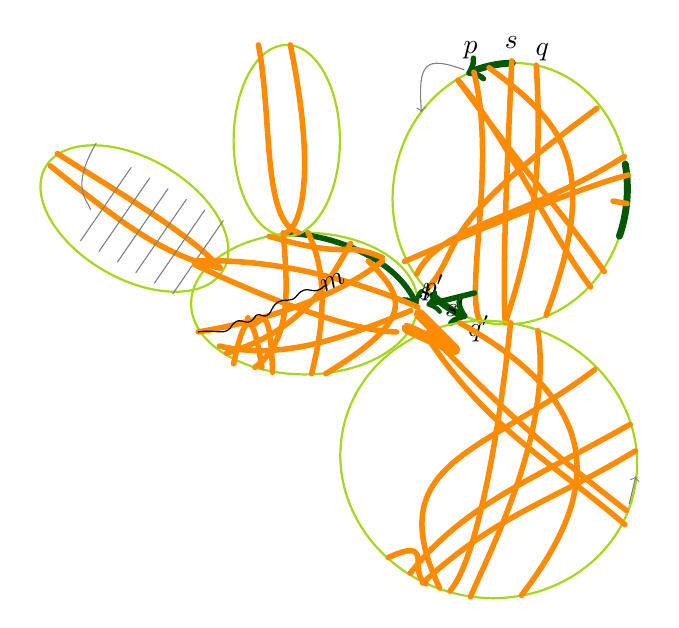
\begin{tikzpicture}[x=.9cm,y=.9cm,line cap=round,line join=round]
\draw[yellow!65!green,thick] (0,0) ellipse(1.6 and 1);
\draw[green!35!black,line width=2pt,->] (-.2,.99)..controls(.5,.95)and(1.3,.6)..(1.59,-.03);
\begin{scope}[shift={(-2.4,1.2)},rotate=-30]
\draw[yellow!65!green,thick] (0,0) ellipse(1.45 and .85);
\draw[orange!90!yellow,line width=2pt] (-1.4,.25)..controls(-.2,.2)and(.8,.2)..(1.4,0) (-1.4,.05)..controls(-.1,-.15)and(.6,-.25)..(1.4,0);
\foreach \x in {-.5,-.2,.1,.4,.7,1}{\draw[gray] (\x,-.65)--({\x+.1},.6);}
\draw[gray] (-1,.65)..controls(-1,-.1)and(-.7,-.1)..(-.6,-.2);
\end{scope}
\draw[yellow!65!green,thick] (-.25,2.3) ellipse(.75 and 1.35);
\draw[orange!90!yellow,line width=2pt] (-.65,3.65)..controls(-.45,2.6)and(-.6,1.15)..(-.08,1) (-.2,3.65)..controls(.1,2.2)and(.05,1.2)..(-.25,1);
\draw[orange!90!yellow,line width=2pt] (-1.55,.6)..controls(-.4,.65)and(.8,.3)..(1.6,-.05) (-1.55,.55)..controls(-.5,.05)and(.7,-.4)..(1.3,-.4);
\draw[orange!90!yellow,line width=2pt] (-.5,.95)..controls(.7,.6)and(.5,.9)..(1.1,.65) (-.3,1)..controls(-.25,.3)and(-.15,-.5)..(-.7,-.9) (.05,1)..controls(.4,.3)and(.2,-.6)..(.1,-.99);
\draw[orange!90!yellow,line width=2pt] (-1.5,-.4)..controls(-.3,-.2)and(.6,.2)..(1.1,.6) (-1.2,-.6)..controls(-.3,-.8)and(.5,-.5)..(1.5,-.1) (-1.1,-.7)..controls(-.1,-.4)and(.3,.2)..(.65,.85);
\draw[orange!90!yellow,line width=2pt] (-1,-.85)..controls(-.8,.1)and(-.7,-.3)..(-.6,-.9) (-.45,-.97)..controls(-.5,.4)and(-.7,-.6)..(-.8,-.2) (.3,-.99)..controls(1.6,-.2)and(1.4,.1)..(.9,.6);
\draw[black,line width=.45pt] (-1.5,-.4)..controls(-1.25,-.36)and(-1.15,-.45)..(-1.05,-.35)..controls(-.92,-.12)and(-.84,-.35)..(-.72,-.22)..controls(-.64,-.05)and(-.56,-.3)..(-.46,-.08)..controls(-.35,.14)and(-.19,-.03)..(-.1,.12)..controls(.05,.3)and(.12,.08)..(.28,.25);
\node[rotate=25] at(.4,.3){$\unsure{m}$};
\begin{scope}[shift={(2.9,1.55)},rotate=-10]
\draw[yellow!65!green,thick] (0,0) ellipse(1.65 and 1.85);
\draw[green!35!black,line width=2.5pt,->] (100:1.65 and 1.85) arc(100:123:1.65 and 1.85);
\draw[green!35!black,line width=2.5pt] (-10:1.65 and 1.85) arc(-10:22:1.65 and 1.85);
\draw[green!35!black,line width=2.5pt,->] (-120:1.65 and 1.85) arc(-120:-100:1.65 and 1.85);
\draw[orange!90!yellow,line width=2pt] (-.8,1.6)..controls(-.25,.4)and(-.4,-1.5)..(-.1,-1.85) (-.3,1.85)..controls(-.1,.3)and(.1,-1.2)..(.25,-1.8) (.05,1.85)..controls(.45,.2)and(.4,-.8)..(.25,-1.8);
\draw[orange!90!yellow,line width=2pt] (-1,1.45)..controls(-.2,.8)and(.6,-.4)..(1.35,-1.1) (-.6,1.7)..controls(.6,1.1)and(1.2,.6)..(.8,-1.6);
\draw[orange!90!yellow,line width=2pt] (-1.1,-1.35)..controls(-.9,-.6)and(.3,-.3)..(1.5,.8) (-1.3,-1.2)..controls(-1,-1)and(1,.3)..(1.6,.55) (-.9,-1.5)..controls(-.5,-.8)and(-1,-.7)..(1,1.4);
\draw[orange!90!yellow,line width=2pt] (-1,1.45)..controls(.3,.2)and(.8,-.15)..(1.5,-.85);
\draw[orange!90!yellow,line width=2pt] (1.45,.15)--(1.65,.15);
\node at(-.9,1.9){$p$};\node at(-.35,2.1){$\unsure{s}$};\node at(.1,2.05){$q$};
\node at(-.83,-1.5){$\unsure{p'}$};\node at(-.48,-1.7){$\unsure{s'}$};\node at(-.1,-1.95){$\unsure{q'}$};
\end{scope}
\begin{scope}[shift={(2.6,-2.2)},rotate=-12]
\draw[yellow!65!green,thick] (0,0) ellipse(2.1 and 1.95);
\draw[orange!90!yellow,line width=2pt] (-.1,1.95)..controls(.05,.6)and(.15,-1.4)..(-.15,-1.93) (.3,1.92)..controls(.8,.6)and(.3,-1.2)..(.15,-1.95);
\draw[orange!90!yellow,line width=2pt] (-1.2,1.58)..controls(-.1,.8)and(.8,.3)..(2.05,-.3) (-1.25,1.55)..controls(-.1,.4)and(.9,.15)..(2.07,-.5);
\draw[orange!90!yellow,line width=2pt] (-.8,1.8)..controls(1.65,1.05)and(1.55,-.3)..(.85,-1.78);
\draw[orange!90!yellow,line width=2pt] (-1.1,-1.65)..controls(-.5,-1.2)and(-.8,-1.8)..(-.5,-1.9) (-.75,-1.8)..controls(-.2,-.7)and(.6,-.2)..(1.85,.9) (-.55,-1.9)..controls(.3,-.7)and(1,-.4)..(2, .55) (-.3,-1.92)..controls(-1.5,-.35)and(-.1,.05)..(1.2,1.55);
\draw[gray,->] (2.07,-.2)--(2.08,.2);
\end{scope}
\draw[orange!90!yellow,line width=4pt] (1.62,-.15)--(2.12,-.65) (1.45,-.35)--(2.1,-.65);
\draw[green!35!black,line width=2pt,->] (2.4,.15)--(1.72,-.02);
\node at(1.7,.14){$\unsure{s}$};
\draw[gray,->] (2.25,3.3)..controls(1.7,3.5)and(1.6,3.4)..(1.65,2.7);
\end{tikzpicture}}

\diagram{\begin{array}{rll}
\texttt{1}&\texttt{//CRAY2\quad JOB\quad '\unsure{*********|**********},\qquad ',',\qquad ',}&\texttt{JOB 0352}\\
&\texttt{// MSGLEVEL=(1,1),MSGCLASS=A}&\\
\texttt{2}&\texttt{// EXEC CSSBATCH}&\\
\texttt{3}&\texttt{XXCSSBATCH PROC REG=100K,P=''}&\texttt{00010000}\\
\texttt{4}&\texttt{XXCSSBATCH EXEC PGM=CRBATCH,REGION=\&REG,PARM=\&P}&\texttt{00020000}\\
\texttt{5}&\texttt{XXSTEPLIB DD DSN=CISI.PROD.CSSBATCH.V1.YY01,DISP=SHR}&\texttt{00030003}\\
\texttt{6}&\texttt{XXSYSUT1 DD DSN=\&\&SYSUT1,UNIT=\unsure{SYSTSO|SYSTS0},SPACE=(TRK,30),DISP=(NEW,DELETE)}&\texttt{00031006}\\
\texttt{7}&\texttt{XXSYSUDUMP DD SYSOUT=*}&\texttt{00040000}\\
\texttt{8}&\texttt{XXCRJIF DD DSN=SYS1.CR.JIF,DISP=SHR}&\texttt{00050000}\\
\texttt{9}&\texttt{XXSYSIN DD DDNAME=CRAYIN}&\texttt{00060000}\\
\texttt{10}&\texttt{//CRAYIN DD *}&
\end{array}}
